
\documentclass[10pt,a4paper]{article}
\usepackage[utf8]{inputenc}
\usepackage[french]{babel}
\usepackage[left=2cm,right=2cm,top=2cm,bottom=2cm]{geometry}
\usepackage{hyperref}

\usepackage{graphicx}

%opening
\title{Rapport d'avancement Projet}
\author{Nicolas Vadkerti et Nathan Lys}
\usepackage{listings} % Required for inserting code snippets
\usepackage[usenames,dvipsnames]{color} % Required for specifying custom colors and referring to colors by name

\definecolor{DarkGreen}{rgb}{0.0,0.4,0.0} % Comment color
\definecolor{highlight}{RGB}{255,251,204} % Code highlight color

\lstdefinestyle{Style1}{ % Define a style for your code snippet, multiple definitions can be made if, for example, you wish to insert multiple code snippets using different programming languages into one document
language=Perl, % Detects keywords, comments, strings, functions, etc for the language specified
backgroundcolor=\color{highlight}, % Set the background color for the snippet - useful for highlighting
basicstyle=\footnotesize\ttfamily, % The default font size and style of the code
breakatwhitespace=false, % If true, only allows line breaks at white space
breaklines=true, % Automatic line breaking (prevents code from protruding outside the box)
captionpos=b, % Sets the caption position: b for bottom; t for top
commentstyle=\usefont{T1}{pcr}{m}{sl}\color{DarkGreen}, % Style of comments within the code - dark green courier font
deletekeywords={}, % If you want to delete any keywords from the current language separate them by commas
%escapeinside={\%}, % This allows you to escape to LaTeX using the character in the bracket
firstnumber=1, % Line numbers begin at line 1
frame=single, % Frame around the code box, value can be: none, leftline, topline, bottomline, lines, single, shadowbox
frameround=tttt, % Rounds the corners of the frame for the top left, top right, bottom left and bottom right positions
keywordstyle=\color{Blue}\bf, % Functions are bold and blue
morekeywords={}, % Add any functions no included by default here separated by commas
numbers=left, % Location of line numbers, can take the values of: none, left, right
numbersep=10pt, % Distance of line numbers from the code box
numberstyle=\tiny\color{Gray}, % Style used for line numbers
rulecolor=\color{black}, % Frame border color
showstringspaces=false, % Don't put marks in string spaces
showtabs=false, % Display tabs in the code as lines
stepnumber=5, % The step distance between line numbers, i.e. how often will lines be numbered
stringstyle=\color{Purple}, % Strings are purple
tabsize=2
}

\newcommand{\insertcode}[2]{\begin{itemize}\item[]\lstinputlisting[caption=#2,label=#1,style=Style1]{#1}\end{itemize}} 


% \insertcode{"Scripts/example.pl"}{Nena would be proud.} 

\begin{document}

\maketitle


\url{https://github.com/SlaynPool/PROJET_IDO/}
\section{Sommaire}
\begin{itemize}
\item Introduction
\item Matériel utilisé
\item Un moteur Brushless
\item Les ESC.
\item Controle d'un moteur
\item Test du moteur
\item Pour plus tard
\item Documentation
\end{itemize}
\section{Introduction}
Cette semaine, nous avons cherché à comprendre et maitriser le controle des moteurs Brushless, qui sont les moteurs couraments utilisés dans l'aeromodelisme. L'idée à donc était de comprendre comment utilisé un moteur brushless, de comprendre le fonctionnement d'un "Electronique Speed Control", ESC, et d'etre capable de controler le moteur, via un microcontroleur.
\section{ Materiel}
\begin{itemize}
 \item Arduino Uno
 \item 4 Afro ESC 20A
 \item 4 Turnigy Multistar 2216-800kv v2
 
\end{itemize}
\section{ Un moteur brushless}
Les moteurs brushless, ou moteur sans balais, sont des moteurs qui comparée aux moteurs à charbon, offrent de bien meilleurs perfomances, que ce soit en terme de couple, d'évacution thérmique donc moins sensible à la chauffe. De plus, il sont bien plus solide que les moteurs à charbon. Voici le schema d'un moteur brushless : 

\begin{figure}[h!]
\centering
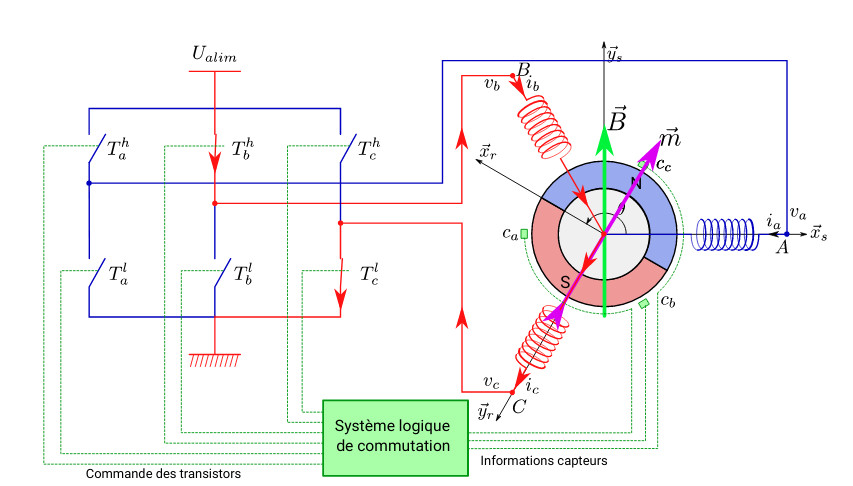
\includegraphics[scale=0.250]{image/1.jpg}
\caption{fonctionnement d'un moteur}
\label{fig:net }
\end{figure}
Le "problème" de ce type de moteur est qu'ils sont difficiles à controler directement. En effet, il faudrait générer trois signals sinusoidales avec des puissances précises ainsi que des déphasages très précis pour exploiter completement le moteur. C'est pour cela que nous allons nous servir d'ESC pour les controler .

\section{Les ESC}
 Comme ennoncé précedement, l'ESC aura donc pour objectif de controler notre moteur, et ainsi nous "simplifier" le controle de celui ci. Il existe plusieurs protocoles numeriques pour communniquer avec L'ESC. Cependant, le plus pratique est d'utiliser un signal PWM. Le PWM est la solution la plus pratique car il est très simple de généré un signal PWM grâce à un Arduino. I
\section{Controle d'un moteur}
Une fois le moteur relié à l'ESC, on peut commencer à controler le moteur, pour les ESC dont on dispose, on utilise la modulation PWM (Modulation à largeur d'impulsion). Durant notre phase de test on a simplement alimenté l'ESC, avec une alimentation réglé sur 14,8V (comme notre batterie). Nous avons ensuite, identifié sur la documentation de l'esc, le pin "SIGNAL", et relié celui ci à un pin de l'arduino capable de généré un PWM (3,5,6,10 et 11). 

Voici le code utilisé pour tester le moteur grâce à la librarie `Servo.h` :
\insertcode{code/1.ino}{Code basique pour controller des moteurs}

 On peut également utiliser la fonction `writeMicroseconds(usec)` afin d'avoir une meilleure préçision pour la puissance utilisé. On va donc avoir de 1060usec à 1430usec pour faire tourner notre moteur. Soit un total de 350 valeurs différentes, à la place de 72 pour la fonction `write`. On va donc utilisé celle-ci sachant qu'elle est plus préçise.

\section{Explication pour la limite du moteur de 12 à 84}
Lorsque l'on "attach" le moteur à un pin, on lui donne 1000us et 2000us. Sur la documentation de l'ESC on nous spécifie 1060us et 1860us. Si on fait un produit en croix entre les valeurs dont on dispose on a :\\

\begin{tabular}{|l|l|}
    Période  & Angle  \tabularnewline    \hline
    1000  & 0  \tabularnewline    \hline
    1060  & 12,6 \tabularnewline    \hline
    1430  & 84,6  \tabularnewline    \hline
    2000  & 180  \tabularnewline    \hline
    
   
        
 \end{tabular}
 \section{Test du moteur}
 Pour tester notre Combo ESC/Moteur, nous avons crée un "banc de test". Celui-ci nous a permis d'utiliser le moteur facilement, en sécurité, ainsi que de faire test sur le poid qu'il peut soulever. Nous avons donc dessiner un banc pour tester notre moteur et construit grâce à la découpeuse laser: \\
 \begin{figure}[h!]
\centering
\includegraphics[scale=0.10]{image/2.jpg}
\caption{Banc de Test}
\label{fig:net }
\end{figure}\\
\url{https://www.youtube.com/watch?v=S_VZyjie2YE}\\
Comme on peut le voir sur la video ci dessus,  nous arrivons à piloter le moteur en variant la vitesse de rotation. Nous avons même pu faire une estimation du poids que celui ci etait capable de soulever à plein puissance. La platforme où est fixer le moteur pèse 500g et le contrepoid 1,50 kg, un seul de nos moteurs peut donc soulever 1kg donc si nous construisons un Quadcoptère nous pourrons theoriquement soulever 4kg.

\section{Suite du Projet}
La prochaine étape de notre projet sera d'écrire le code permettant de faire voler le drone. On pourra trouver un moyen de communication pour diriger/ envoyer des ordres au drone. On pourra également se servir de la fonction `read` afin de savoir dans quel état se trouve le moteur.

\section{Documentation/source}
\begin{itemize}
 \item Fonction de la librairie Servo.h :\\
\url{https://www.arduino.cc/en/Reference/Servo}
\item Video du banc de test en activité : \\
\url{https://www.youtube.com/watch?v=S_VZyjie2YE}
\item Moteur : \\
\url{https://cdn-global-hk.hobbyking.com/media/file/288905599X28019X33.pdf}
\item ESC :\\
\url{https://www.flyingtech.co.uk/sites/default/files/product_files/AfroESC\%2020A\%20USER\%20MANUAL\_0.pdf}
\end{itemize}







\end{document}

